% submit to https://sites.google.com/site/wpmvp2014/home
\documentclass[10pt, onecolumn, preprint]{sigplanconf}

% The following \documentclass options may be useful:

% preprint      Remove this option only once the paper is in final form.
% 10pt          To set in 10-point type instead of 9-point.
% 11pt          To set in 11-point type instead of 9-point.
% authoryear    To obtain author/year citation style instead of numeric.

\usepackage{amsmath}
\usepackage{listings}
\usepackage{hyperref}

\special{papersize=8.5in,11in}
\setlength{\pdfpageheight}{\paperheight}
\setlength{\pdfpagewidth}{\paperwidth}

%\conferenceinfo{WPMVP '14}{February 16, 2014, Orlando, FL, USA} 
%\copyrightyear{2014} 
%\copyrightdata{978-1-4503-2653-7/14/02}
%\doi{2568058.2568060}

\lstset{captionpos=b, float, language=python}

\usepackage{tikz}
\usetikzlibrary{positioning}
\usetikzlibrary{shadows}
\usetikzlibrary{arrows}
\usetikzlibrary{shapes}

\providecommand{\boostsimd}{\textsc{Boost.SIMD}}
\providecommand{\cpp}[1][~]{\textsc{C++}#1}
\providecommand{\ie}[1][~]{\textit{i.e.}#1}
\providecommand{\eg}[1][~]{\textit{e.g.#1}}


\begin{document}


\title{Pythran: Enabling Static Optimization of Scientific Python Programs}

\authorinfo{Serge Guelton}
           {T{\'e}l{\'e}com Bretagne}
           {serge.guelton@telecom-bretagne.eu}
\authorinfo{Pierrick Brunet}
           {INRIA/MOAIS}
           {pierrick.brunet@inria.fr}
\authorinfo{Mehdi Amini}
           {SILKAN}
           {mehdi.amini@silkan.com}
\authorinfo{Adrien Merlini}
           {T{\'e}l{\'e}com Bretagne}
           {adrien.merlini@telecom-bretagne.eu}
\authorinfo{Xavier Corbillon}
           {T{\'e}l{\'e}com Bretagne}
           {xavier.corbillon@telecom-bretagne.eu}
\authorinfo{Alan Raynaud}
           {T{\'e}l{\'e}com Bretagne}
           {alan.raynaud@telecom-bretagne.eu}

\maketitle

\begin{abstract}

    Pythran is an open source static compiler that turns modules written in a
    subset of Python language into native ones. Assuming that scientific
    modules do not rely much on the dynamic features of the language, it trades
    them for powerful, possibly inter procedural, optimizations.  These
    optimizations include detection of pure functions, temporary allocation
    removal, constant folding, Numpy \texttt{ufunc} fusion and parallelization,
    explicit thread-level parallelism through OpenMP annotations, false
    variable polymorphism pruning, and automatic vector instruction generation
    such as AVX or SSE.

    In addition to these compilation steps, Pythran provides a C++ runtime 
    library that
    leverages the C++ STL to provide generic containers, and the Numeric 
    % FIXME (phrase trop longuuuuuuuuue) 
    Template Toolbox (NT2) for Numpy support. It takes advantage of modern C++11
    features such as variadic templates, type inference, move semantics and
    perfect forwarding, as well as classical idioms such as expression templates.

    % FIXME  (explain that annotations can be added to the code?)
    Unlike the Cython approach, Pythran input code remains compatible with the
    Python interpreter. Output code is generally as efficient as the annotated
    Cython equivalent, if not more, but without the backward compatibility
    loss.


\end{abstract}


\keywords
static compilation, parallelization, Python, C++


%%
%%
\section{Introduction}

The Python language is growing in popularity as a language for scientific
computing, thanks to % FIXME (sounds strange for a publication) its concise
syntax, a high level standard library and several scientific packages. The
combination of a relatively efficient array package --\texttt{numpy}--, a
library for scientific computing --\texttt{scipy}--, and enhanced interactive
console --\texttt{ipython}-- and a comprehensive 2D plotting package
--\texttt{matplotlib}-- makes it a relevant candidate for many daily scientific
tasks.

However, the overhead of running a scientific application written in Python
compared to the same algorithm written in a statically compiled language such
as C is high. It is partly due to the interpretation cost, but also to Python's
dynamic binding. Additionally, the Python compiler does not perform any
optimization on the byte code, while scientific applications are first-class
candidates for many of them. The ratio between an efficient C application and
its Python counterpart can range from a factor of two, when the Python code
only calls C routine, to a factor of one hundred or more when the Python code
makes explicit array accesses.

Given the increasing amount of data that scientists may need to process for
their experiments, even two can be a limiting factor for the adoption of Python
for computation intensive experiments. But since scientific applications are
often told to spend 90\% of their time in 10\% of the code, one can focus on
those computation-intensive pieces of code. The goal of an optimizing compiler
may not be to optimize the full Python application, but rather a subset of the
application.

Several tools have been developed by an active community to fill the performance
gap encountered when running these computation-intensive piece of code, either
% FIXME after? (perfs issues are not on the compilation (except for...))
through static compilation or Just In Time (JIT) compilation.

One approach, used by Cython~\cite{cython2010} is to suppress the interpretation
overhead by translating Python Programs to C programs calling the Python C
API~\cite{pythoncapi}. More recently, Nuitka~\cite{nuitka}  has taken the same
approach using C++ as a back-end. Going a step further Cython also provides an
hybrid C/Python language that can efficiently be translated into C code. It 
relies both on the Python C API and on plain C.
ShedSkin~\cite{shedskin2006} translates implicitly strongly typed Python programs
into C++, without any call to the Python C API, but fails to compile dynamic
codes or codes for which static type inference is impossible.

The alternate approach consists in writing a JIT compiler, embedded into the
interpreter, to dynamically turn the computation intensive parts into native
code. This is what the \texttt{numexpr} module~\cite{numexpr} does for Numpy 
expressions, JIT-compiling them from a string representation to native code.
Numba~\cite{numba} and Parakeet~\cite{parakeet2012} extend this approach to
Numpy-centric applications while PyPy~\cite{pypy2009} applies it to the whole
language - including the Numpy module through the in-progress \texttt{numpypy}
branch.

Except for PyPy, none of these compilers apply any of the static optimization
techniques that have been known and successfully applied 
% FIXME And Numba? It generates LLVM, which uses static optimization techniques
for decades to statically compiled language such as C or C++.  Translators to
statically compiled languages do take advantage of them indirectly, but the
quality of the generated code may prevent advanced optimizations. For instance
GCC hardly vectorizes the output of Cython, while the array semantic is
available at the Python level. Taking into account the specificities of the
Python language can unlock many new transformations.  For instance, PyPy
automatically converts the \texttt{range} builtin into \texttt{xrange} by using
a dedicated structure called \texttt{range-list}.

This article presents Pythran, an optimizing compiler for a subset of the
Python language that turns implicitly statically typed modules into parametric
C++ code. It supports many high-level constructs of the 2.7 version of the
Python language such as list comprehension, set comprehension, dict
comprehension, generator expression, lambda functions, nested functions,
polymorphic functions and global variables. It does \textbf{not} support user
classes or any dynamic feature such as introspection or polymorphic variables.

Unlike existing alternatives, Pythran does not solely perform static typing of
Python programs. It also performs various compiler optimizations such as
detection of pure functions, temporary allocation removal or constant folding.
These transformations are backed up by code analyses such as aliasing,
inter-procedural memory effect computations or use-def chains.

The article is structured as follows: Section~\ref{sec:infrastructure}
introduces the Pythran compiler compilation flow and internal representation.
Section~\ref{sec:analysis} presents several code analyses while
Section~\ref{sec:optimizations} focuses on code optimizations.
Section~\ref{sec:backend} presents back-end optimizations for Numpy
expressions. Section~\ref{sec:openmp}  briefly introduces OpenMP-like
annotations for explicit parallelization of Python programs and
Section~\ref{sec:benchmarks} presents the performance obtained on a few
synthetic benchmarks and concludes.


\section{Pythran Compiler Infrastructure}
\label{sec:infrastructure}

Pythran is a compiler for a subset of the Python language. In this paper, the
name \textbf{Pythran} will be used indifferently to refer to the language or
the associated compiler. The input of the Pythran compiler is a Python module
---not a Python program--- meant to be turned into a native module. Typically,
computation-intensive parts of the program are moved to a module fed to
Pythran. The module is then translated to polymorphic C++ code through the
generation of templated classes in place of Python functions. These classes are
either used from regular C++ applications, or instantiated for given types to
generate a native Python module.

It is a strong requirement for Pythran to maintain backward compatibility with
Python, that is, unlike Cython, all code compilable by Pythran is still
executable by a standard-conforming Python interpreter. For this reason, in
addition to language restrictions detailed in the following, Pythran
understands special comments such as:

\begin{lstlisting}
#pythran export foo(int list, float)
\end{lstlisting}

as an optional module signature. One does not need to list all the module
functions in an \texttt{export} directive, only the functions meant to be used
outside of the module, i.e imported by another module.
Polymorphic functions can be listed several times with
different types. These type annotations are only used for native code generation.

The Pythran compiler is built as a traditional static compiler: a front-end
turns Python code into an Internal Representation (IR), a middle-end performs
various code optimizations on this IR, and a back-end turns the IR into C++
code. The front-end performs two steps:

\begin{enumerate}

    \item turn Python code into Python Abstract Syntax Tree (AST) by using the \texttt{ast}
   module from the standard library;

    \item turn the Python AST into a type-agnostic Pythran IR, which remains a subset
   of the Python AST.

\end{enumerate}

Pythran IR is similar to the Python AST, as defined in the \texttt{ast} module, except
that several nodes are forbidden (for instance because Pythran does not support
user-defined classes, or the \texttt{exec} instruction), and some nodes are converted
to others to form a simpler and easier to deal with AST for further analyses and
optimizations. The transformations applied by Pythran on Python AST are the
following:

\begin{itemize}
    \item list/set/dict comprehension are expanded into loops wrapped into a function call;

    \item destructuring is expanded into several variable assignments;

    \item lambda functions are turned into named nested functions;

    \item the closure of nested functions is statically computed to turn nested
        functions into global functions taking the closure elements as
        parameters. The initial definition is replaced by a \emph{partial
        function} creation, using the \texttt{partial} type from the standard \texttt{functools} module;

    \item implicit \texttt{return None} are made explicit;

    \item all imports are fully expanded to make functions and global variables access paths explicit,

    \item method calls are turned into function calls;

    \item implicit \texttt{\_\_builtin\_\_} function calls are made explicit;

    \item \texttt{try \dots finally} instriuction are turned into nested \texttt{try \dots except} instructions;

    \item identifiers whose name may be in conflict with C++ keywords are renamed.

\end{itemize}

The back-end operates in three steps:

\begin{enumerate}

    \item turning Pythran IR into parametric C++ code;

    \item instantiating the C++ code for the desired types;

    \item compiling the generated C++ code into native code.

\end{enumerate}

The first step requires to map polymorphic variables and polymorphic functions
from the Python world to C++. Pythran only supports polymorphic variables for
functions, i.e. a variable can hold several function objects during its life
time, but it cannot be assigned to a string if it has already been assigned to
an integer.  As shown later, it is possible to detect several false variable
polymorphism cases using use-def chains. Function polymorphism is achieved
through template parameters: a template function can be applied to several
types as long as an implicit structural typing is respected. This technique is
very similar to Python's duck typing, except that it is checked at compile
time, as illustrated by the following implementation of a generic dot product
in Python:

\begin{lstlisting}
def dot(L0, L1):
    return sum(x*y for x,y in zip(L0,L1))
\end{lstlisting}

\noindent and in C++:

\begin{lstlisting}[language=c++]
template<class T0, class T1>
    auto dot(T0&& L0, T1&& L1) -> decltype(/* skipped */)
    {
        return pythonic::sum(
            pythonic::map(
                operator_::multiply(),
                    pythonic::zip(
                        std::forward<T0>(L0),
                        std::forward<T1>(L1))
            )
        );
    }
\end{lstlisting}

Although more verbose than the Python version, the C++ version also uses some
form of structural typing: the only assumptions these two versions make are
that \texttt{L0} and \texttt{L1} are iterable, their content can be multiplied
and that the result of the multiplication is accumulatable.

Finally, Pythran computes the set of functions and types used for the processed
module, and generates the minimal set of headers that provide the definitions
needed to compile the generated C++ code. This step is critical to prevent
typical slowdown during C++ compilation.

The second step only consists in the instantiation of the top-level functions
of the module, using user-provided signatures. Template instantiation then
triggers the different correctly typed instantiations for all functions called
in the module. Note that the user only needs to provide the type of the
functions exported outside the module. The possible types of all internal
functions are then inferred from the call sites. This complex step leverage the
C++11 compiler capabilities: Pythran generates only one line using
user-provided signature to trigger the template instanciation by the C++
compiler.

The last step involves a template library, called \texttt{pythonic} that 
contains a polymorphic implementation of many functions of the Python standard
library in the form of C++ template functions. Several optimizations, most
notably using expression templates, are delegated to this library. Pythran relies
on the C++11~\cite{isocxx11} language and leverages recent features such as
move semantics, type inference through \texttt{decltype(\dots)} and variadic
templates.
As a consequence it requires a C++11 compatible compiler for the native code
generation. Boost.Python~\cite{boostpython2007} is used for the automatic
Python-to-C++ boilerplate. Generated C++ code is compatible starting with g++ 
4.8.2 and clang++ 3.3.

It is important to note that all Pythran analyses and optimizations are
type-agnostic, \ie{they do not assume any type for the variables manipulated
by the program}. The specialization of the generated code occurs only by generating the template instanciation.
In other words, the Pythran compiler analyzes polymorphic functions and turns
Python modules into C++ meta-programs.

Figure~\ref{fig:pythran-compiler} summarizes the compilation flow and the 
involved tools.

\begin{figure}

    \centering
    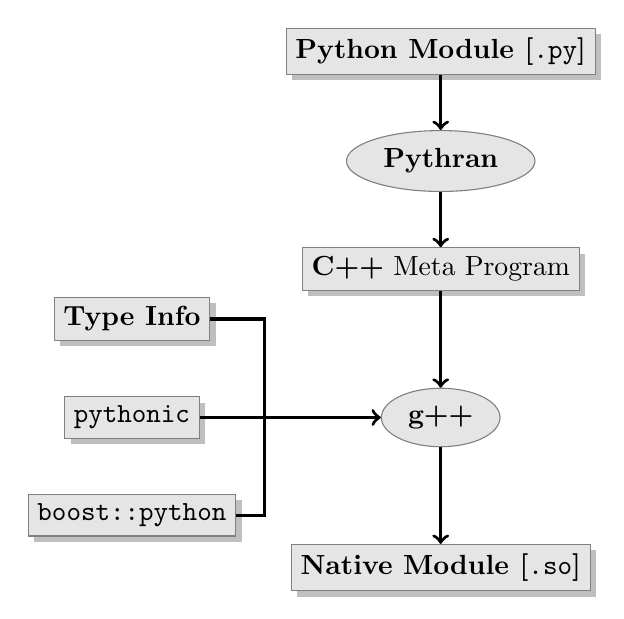
\begin{tikzpicture}[
            file/.style={draw=black!50,fill=black!10,rectangle, drop shadow, align=center,
            node distance=0.7cm},
            tool/.style={draw=black!50,fill=black!10,ellipse, align=center, node
        distance=0.7cm}]
        \node[file] (python) {\textbf{Python Module [\texttt{.py}]}};
        \node[tool] (pythran) [below=of python] {\textbf{Pythran}};
        \node[file] (meta-cxx) [below=of pythran] {\textbf{C++} Meta Program};
        \node[tool] (gxx) [yshift=-1.5em, below=of meta-cxx] {\textbf{g++}};
        \node (empty) [xshift=-1em, left=of gxx] {};
        \node[file] (pythonic) [left=of empty] {\textbf{\texttt{pythonic}}};
        \node[file] (annotation)     [above=of pythonic] {\textbf{Type Info}};
        \node[file] (boost) [below=of pythonic] {\textbf{\texttt{boost::python}}};
        \node[file] (so) [yshift=-1.5em, below=of gxx] {\textbf{Native Module [\texttt{.so}]}};

        \draw[very thick, ->] (python) -- (pythran);
        \draw[very thick] (annotation) -| (empty.center);
        \draw[very thick, ->] (pythran) -- (meta-cxx);
        \draw[very thick, ->] (meta-cxx) -- (gxx);
        \draw[very thick] (boost) -| (empty.center);
        \draw[very thick, ->] (pythonic) -- (gxx);
        \draw[very thick, ->] (gxx) -- (so);
    \end{tikzpicture}
    
    \caption{Pythran compilation flow.}
    \label{fig:pythran-compiler}

\end{figure}



\section{Code Analyses}
\label{sec:analysis}

A code analysis is a function that takes a part of the IR (or the whole
module's IR) as an input and returns aggregated high-level information. For
instance, a simple Pythran analysis called \texttt{Identifiers} gathers the set
of all identifiers used throughout the program. This information is later used
when creating new identifiers so that no conflict occurs with already existing ones.

One of the most important analysis in Pythran is the \textbf{alias analysis}, sometimes
referred as \textbf{points-to} analysis. For each identifier, it computes an
approximation of the set of locations this identifier may points to. For
instance, let us consider the polymorphic function \texttt{foo} defined as follows:

\begin{lstlisting}
def foo(a,b):
    c = a or b
    return c * 2
\end{lstlisting}

The identifier \texttt{c} involved in the multiplication may refer to

\begin{itemize}
    \item a fresh location if \texttt{a} and \texttt{b} are scalars

    \item the same location as \texttt{a} if \texttt{a} evaluates to \texttt{True}

    \item the same location as \texttt{b} otherwise.

\end{itemize}

As we do not specialise the analysis for different types and the truth value of
\texttt{a} is unknown at compilation time, the alias analysis yields % FIXME (sounds strange) 
the approximated result that \texttt{c} may point to a fresh location, 
\texttt{a} or \texttt{b}.

Without this kind of information, even a simple instruction like
\texttt{sum(a)} would yield very few information as there is no guarantee that
the \texttt{sum} identifiers point to the \texttt{sum} built-in, as it could have been 
previously stated that \texttt{sum = len}.

When turning Python AST into Pythran IR, nested functions are turned into
global functions taking their expanded closure as parameter. This closure is
computed using the information provided by the \texttt{Globals} and
\texttt{ImportedIds} analyse. The former statically computes the state of the
dictionary of globals, and the latter computes the set of identifiers used by
an instruction but not declared in this instruction. For instance in the
following snippet:

\begin{lstlisting}
def outer(outer_argument):
    def inner(inner_argument):
        return cos(outer_argument) + inner_argument
    return inner(3)
\end{lstlisting}

The \texttt{Globals} analysis called on the \texttt{inner} function definition
marks \texttt{cos} as a global variable, and \texttt{ImportedIds} marks
\texttt{outer\_argument} and \texttt{cos} as imported identifiers. The result
of the transformation of nested function into global functions on that
particular example is:

\begin{lstlisting}
import functools

def _inner(outer_argument, inner_argument):
    return cos(outer_argument) + inner_argument

def outer(outer_argument):
    inner = functools.partial(_inner, outer_argument)
    return inner(3)
\end{lstlisting}

A rather high-level analysis is the \texttt{PureFunctions} analysis, that computes the
set of functions declared in the module that are pure, \ie{whose return value
only depends from the value of their arguments and do not change any global state}.
This analysis depends on two
other analyses, namely \texttt{GlobalEffects} that computes for each function whether
it modifies the global state (including I/O, random generators, etc.)
and \texttt{ArgumentEffects} that computes for each argument of each function 
whether or not this argument may be updated in the function body. These three
analyses work inter-procedurally, as illustrated in the following example:

\begin{lstlisting}
def fibo(n):
    return n if n < 2 else fibo(n - 1) + fibo(n - 2)

def bar(l):
    return map(fibo, l)

def foo(l):
    return map(fibo, random.sample(l, 3))
\end{lstlisting}

The \texttt{fibo} function is pure as it has no global effect or argument effect and
only calls itself. As consequence the \texttt{bar} function is also pure since the
\texttt{map} intrinsic is pure when its first argument is pure. However the \texttt{foo}
function is not pure since it calls the \texttt{sample} function from the \texttt{random}
module, which has a global effect (on the underlying random number generator
internal state).

Several analyses depend on the \texttt{PureFunctions} analysis.
\texttt{ParallelMaps} uses aliasing information to check if an identifier
points to the \texttt{map} intrinsic, and checks if the first argument is a
pure function using \texttt{PureFunctions}. In that case the \texttt{map} is
added to the set of parallel maps, because it can be executed in any order.
This is the case for the first \texttt{map} in the following snippet, but not
for the second because \texttt{print b} involves an \textbf{I/O}.
% Which is not really usefull as there is no way to say pythran we want to execut it in parallel
% (but logging information is still displayed)

\begin{lstlisting}
def pure(a):
    return a ** 2

def guilty(a):
    b = pure(a)
    print b
    return b

l = list(...)
map(pure, l)
map(guilty, l)
\end{lstlisting}

\texttt{ConstantExpressions} uses function purity to decide whether or not a given expression
is constant, \ie{its value only depends on literals}. For instance the
expression \texttt{fibo(12)} is a constant expression because \texttt{fibo} is pure and its
argument is a literal. 
% FIXME (pourrait etre interressant de repondre a : et t'en fait quoi calcul a la compilation? calcul une fois si appele plusieurs fois ?... ou ref a la transformation qui fait ca)
% PB : explain later I think.

\texttt{UseDefChains} is a classical analysis from the static compilation world. For
each variable defined in a function, it computes the chain of \textbf{use} and \textbf{def}.
The result can be used to drive various code transformations, for instance to
remove dead code, such as a \textbf{def} followed by either nothing or a 
\textbf{def} is useless. 
It is used in Pythran to avoid false polymorphism. An intuitive way to represent
use-def chains is illustrated on the next code snippet:

\begin{lstlisting}
a = 1
if cond:
    a = a + 2
else:
    a = 3
print a
a = 4
\end{lstlisting}

In this example, there are two possible chains starting from the first
assignment. Using \texttt{U} to denote \textbf{use} and \texttt{D} to denote \textbf{def}, one gets:

\begin{center}
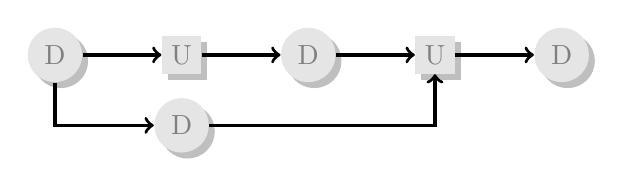
\begin{tikzpicture}[D/.style={black!50,fill=black!10, circle, drop shadow, align=center},
    U/.style={black!50,fill=black!10, rectangle, drop shadow, align=center}]
    \node[D] (d0) {D};
    \node[U] (u0) [right=of d0] {U};
    \node[D] (d1) [right=of u0] {D};
    \node[U] (u1) [right=of d1] {U};
    \node[D] (d2) [right=of u1] {D};

    \node[D] (dp0)[below=of u0, yshift=2em] {D};

    \draw[very thick, ->] (d0) -- (u0);
    \draw[very thick, ->] (d0) |- (dp0);
    \draw[very thick, ->] (u0) -- (d1);
    \draw[very thick, ->] (d1) -- (u1);
    \draw[very thick, ->] (dp0) -| (u1);
    \draw[very thick, ->] (u1) -- (d2);
\end{tikzpicture}
\end{center}

The fact that all paths finish by a \textbf{def} indicates that the last
assignment can be removed (but not necessarily its right hand part that could
have a side-effect). % FIXME example?
In the use-def Chains, we can gather all nodes tied with a \textbf{use} node or
preceded by a common \textbf{def} node.
All these nodes refere to the same variable and can
safely be renamed from \texttt{a} to \texttt{a}' (thus performing scalar
renaming). It avoid false polymorphism.
% FIXME The scalar renaming part is unclear
% PB : Is it clearer now? I don't speak about UD node but we don't care, do we?

All the above analyses are used by Pythran developers to build code
transformations that improve the execution time of the generated code.

\section{Code Optimizations}
\label{sec:optimizations}

One of the benefits of translating Python code to C++ code is that it removes
most of the dynamic lookups. It also unveils all the optimizations available at
C++ level. For instance, a function call is quite costly in Python, which
advocates in favor of using inlining. This transformation comes at no cost when
using C++ as the back-end language, as the C++ compiler performs this 
transformation triggered by fine tuned heuristics.

However, there are some information available at the Python level that cannot
be recovered at the C++ level. For instance, Pythran uses functor with an
internal state and a goto dispatch table to represent generators. This approach
is not very efficient, especially for trivial cases.
Such trivial cases appear when a generator expression is converted, in the
front-end, to a looping generator. To avoid this extra cost, Pythran turns
generator expressions into call to \texttt{imap} and \texttt{ifilter} from the
\texttt{itertools} module whenever possible, removing the unnecessary goto
dispatching table. This kind of transformation cannot be made by the C++
compiler. For instance, the one-liner \texttt{len(set(vec[i]i + i for i in cols))}
extracted from the \texttt{nqueens} benchmarks from the Unladen Swallow project
is rewritten as \texttt{len(set(itertools.imap(lambda i: vec[i] + i,cols)))}.
This new form is less efficient in pure Python (it implies one extra function
call per iteration), but can be compiled into C++ more efficiently than a
generic generator.

A similar optimization consists in turning \texttt{map}, \texttt{zip} or
\texttt{filter} into their equivalent version from the \texttt{itertool}
module. The benefit is twofold: first it removes a temporary allocation, second
it gives an opportunity to the compiler to replace list accesses by scalar
accesses. This transformation is not always valid, nor profitable. It is not
valid if the content of the output list is written later on, and not profitable
if the content of the output list is read several times, as each read implies
the (re) computation, as illustrated in the following code:

\begin{lstlisting}
def valid_conversion(n):
    # this map can be converted to imap
    L = map(math.cos, range(n))
    return sum(L) # sum iterates once on its input

def invalid_conversion(n):
    # this map cannot be converted to imap
    L = map(math.cos, range(n))
    L[0] = 1  # invalid assignment if converted to imap
    return sum(L) + max(L) # two iterations over L prevents imap transformation
\end{lstlisting}

The information regarding constant expressions is used to perform a classical
transformation called \texttt{ConstantFolding}, which consists in the compile-time
evaluation of constant expressions. The validity is guaranteed by the
\texttt{ConstantExpressions} analysis, and the evaluation relies on Python ability to
compile an AST into byte code and run it, benefiting from the fact that Pythran
IR is a subset of Python AST. A typical illustration is the initialization of a
cache at compile-time:

\begin{lstlisting}
def esieve(n):
    candidates = range(2, n+1)
    return sorted(
        set(candidates) - set(p*i
                              for p in candidates
                              for i in range(p, n+1))
        )

cache = esieve(100)
\end{lstlisting}

Pythran automatically detects that \texttt{eseive} is a pure function and evaluates
the \texttt{cache} variable value at compile time.

\texttt{ConstantFolding} may create a lot of candidates for 
\texttt{LoopUnrolling}. In Python, loops are used to iterate over sequences. If
such a sequence is an explicit list, then Pythran unrolls the loop accordingly.
Thanks to \texttt{ConstantFolding}, a call to \texttt{range(4)} will statically
turn into \texttt{[0, 1, 2, 3]} (after a check that \texttt{range} actually
points to \texttt{\_\_builtin\_\_.range}) making it possible to unroll the loop
statically.

Sometimes, developers use the same variable in a function to represent value 
with different types, which leads to false polymorphism, as in:

\begin{lstlisting}
a = cos(1)
a = str(a)
\end{lstlisting}

These instructions cannot be translated to C++ directly because \texttt{a}
would have both \texttt{double} and \texttt{str} type. However, using
\texttt{UseDefChains} it is possible to assert the validity of the renaming of
the instructions into:


\begin{lstlisting}
a = cos(1)
a_ = str(a)
\end{lstlisting}

that does not have the same typing issue.

In addition to these python-level optimizations, the Pythran back end library,
\texttt{pythonic}, uses several well known optimizations, especially for Numpy
expressions.

\section{Library Level Optimizations}
\label{sec:backend}

Using the proper library, the \cpp language provides an abstraction level close
to what Python proposes. Pythran provides a wrapper library, \texttt{pythonic},
that leverage on the \cpp Standard Template Library (STL), the GNU Multiple
Precision Arithmetic Library (GMP) and the Numerical Template Toolbox
(NT2)\footnote{\url{https://github.com/MetaScale/nt2}} to emulate Python
standard library. The STL is used to provide a typed version of the standard
containers (\texttt{list}, \texttt{set}, \texttt{dict} and \texttt{str}), as
well as reference-based memory management through \texttt{shared\_ptr}. Generic
algorithms such as \texttt{accumulate} are used when possible. GMP is the
natural choice to represent Python's \texttt{long} in \cpp. NT2 provides a generic
vector library called \texttt{boost.simd}~\cite{esterie2012boost} that enables
the use of vector instruction units of modern processors in a generic way. It is used
to efficiently compile Numpy expressions.

Numpy expressions are the perfect candidates for library level optimizations.
Pythran implements three optimizations on such expressions:

\begin{enumerate}

    \item Expression templates~\cite{expression_templates} are used to avoid
        multiple iterations and the creation of intermediate arrays. Because
        they aggregate all \texttt{ufunc} into a single expression at compile
        time, they also increase the computation intensity of the loop body,
        and hence increase the impact of the two following optimizations.
        % what about binary func?
        % ufunc -> micro function, in numpy ;-)

    \item Loop vectorization. All modern processors have vector instruction
        units capable of applying the same operation on a vector of data
        instead of a single data. For instance Intel Sandy Bridge can run 8
        single-precision additions per instruction. One can directly use the
        vector instruction set assembly to use these vector units, or use C/C++
        intrinsics. Pythran relies on \texttt{boost.simd} from NT2 that offers
        a generic vector implementation of all standard math functions to
        generate a vectorized version of Numpy expressions. Again, the
        aggregation of operators performed by the expression templates proves
        to be beneficial, as it reduces the number of (costly) loads from the
        main memory to the vector unit.

    \item Loop parallelization through OpenMP~\cite{openmp3.1}. Numpy expression
        computation do not carry any loop-dependency. They are perfect
        candidates for loop parallelization, especially after the expression
        templates aggregation, as OpenMP generally performs better on loops
        with higher computation intensity that masks the scheduling overhead.

\end{enumerate}

To illustrate the benefits of these three optimizations combined, let us
consider the simple Numpy expression:

\begin{lstlisting}
d = numpy.sqrt(b*b+c*c)
\end{lstlisting}

When benchmarked with the \texttt{timeit} module on an hyper-threaded quad-core 
i7, the pure Python execution yields: % FIXME sandy-brige? nehalem?...
% PB : Not sure it is needed as audiance don't really care about it.

\begin{lstlisting}
>>> %timeit np.sqrt(b*b+c*c)
1000 loops, best of 3: 1.23 ms per loop
\end{lstlisting}

\noindent then after Pythran processing and using expression templates:

\begin{lstlisting}
>>> %timeit my.pythranized(b,c)
1000 loops, best of 3: 621 us per loop
\end{lstlisting}

The speed-up is due to the fact that expression templates replace 4 temporary
array creations and 4 loops by a single allocation and a single loop.

Going a step further and vectorizing the generated loop yields an extra
performance boost:

\begin{lstlisting}
>>> %timeit my.pythranized(b,c)
1000 loops, best of 3: 418 us per loop
\end{lstlisting}

Although the AVX instruction set makes it possible to store 4 double precision
floats, one does not get a 4x speed up because of the (unaligned) memory transfers
to and from vector registers.
% 1.33x speedup is not really good if the best expected is 4x. unaligned explain why it is not better 
% than 2x but what about the others 0.66?

Finally, using both expression templates, vectorization and OpenMP:

\begin{lstlisting}
>>> %timeit my.pythranized(b,c)
1000 loops, best of 3: 105 us per loop
\end{lstlisting}

The 4 hyper-threaded cores give an extra performance boost. In the end, Pythran
generates a native module that performs roughly $\times11$ faster than the
original version.

As a reference, the \texttt{numexpr} module that performs JIT optimization of the
expression yields the following timing:

\begin{lstlisting}
>>> %timeit numexpr.evaluate("sqrt(b*b+c*c)")
1000 loops, best of 3: 395 us per loop
\end{lstlisting}

\noindent Pythran still performs almost four times faster.

\section{Explicit Parallelization}
\label{sec:openmp}

Many scientific applications can benefit from the parallel execution of their
kernels. As modern computers generally feature several processors and several
cores per processor, it is critical for the scientific application developers to
be able to take advantage of them.
%Does python programmer really use it? Or people using it may write their native code?
% They may write it using python only to prototyping?

As explained in the previous section, Pythran takes advantage of multiple cores
when compiling Numpy expressions. However, when possible, it is often more
profitable to parallelize the outermost loops rather than the inner loops
---the Numpy expressions--- because it avoids the synchronization barrier at
the end of each parallel section, and generally offers more computation
intensive computations.

The OpenMP standard~\cite{openmp3.1} is a widely used solution for Fortran, C
and C++ to describe loop-based and task-based parallelism. It consists of a few
directives attached to the code, directives that describe parallel loops and parallel code
sections in a shared memory model.

Pythran makes this directives available at the Python level through string
instructions. The semantic is roughly similar to the semantics defined by the
standard, assuming that all variables have function-level scope.

The following listing gives a simple example of explicit loop-based parallelism
(OpenMP 3.0 task-based parallelism form is also supported, the interested
reader may refer to~\cite{pyhpc2013} for more details). the \texttt{kernel}
function is pure and computation intensive, making the loop a perfect candidate
for parallelization. 

\begin{lstlisting}
def compute_julia(cr, ci, N, bound=1.5, lim=1000., cutoff=1e6):
    julia = np.empty((N, N), np.uint32)
    grid_x = np.linspace(-bound, bound, N)
    #omp parallel for 
    for i, x in enumerate(grid_x):
        for j, y in enumerate(grid_x):
            julia[i,j] = kernel(x, y, cr, ci, lim, cutoff)
    return julia
\end{lstlisting}

As in in standard OpenMP, loop indices of the parallel loop are automatically
made private, and Pythran extends the concept to any random access iterator,
even after type destructuring. In the example, both \texttt{i} and \texttt{x}
are private. A scope analysis is used to prove that \texttt{j} and \texttt{y}
are also local to the loop. In the end, the whole computation achieves a
perfect speedup of $\times4$

Next section performs an in-depth comparison of Pythran with three other Python
optimizers: CPython, Cython and PyPy.

\section{Benchmarks}
\label{sec:benchmarks}


All benchmarks presented in this section are run on an hyper-threaded quad-core
i7, % FIXME sandy-brige, nehalem, what?
using examples shipped along with
Pythran sources, available at \url{https://github.com/serge-sans-paille/pythran} in
the \texttt{pythran/test/cases} directory. The Pythran version used is the
\texttt{HEAD} of the \texttt{iop2014} branch. The other tools are: PyPy 2.0.2 compiled with the
\texttt{-jit} flag, CPython 2.7.3 and Cython 0.20. All timings are made using
the \texttt{timeit} module, taking the best of all runs. All C++ codes are
compiled with g++ 4.8.2, using the tool default compiler option, generally
\texttt{-O3} plus a few optimizing flags depending on the target. To make a
fair comparison, no parallelism annotations are added to any code.

Provided each module has been properly compiled, each experiment is run using
the following command from a shell:

\begin{lstlisting}[language=sh]
python -m timeit -s "${SETUP}" "${RUN}"
\end{lstlisting}

\noindent where \texttt{\$SETUP} and \texttt{\$RUN} depend on the benchmark and
\texttt{pypy} is substituted to \texttt{python} when needed. The
\texttt{\$SETUP} and \texttt{\$RUN} values are available to the reader on the
Git repository in the \texttt{doc/papers/iop/xp/run\_benchamrks.sh} file with
all the experimental setup.

The same source is used for each benchmark, to the exception of Cython sources
which needed a manual conversion. For these sources, bound checking and wrap
around are always disable, all variables are declared using the proper C or C++
type and all mathematical functions in use come from \texttt{libm}. Some calls
to the \texttt{zeros\_like} function also have been replaced by calls to
\texttt{zeros} for the PyPy version.

\subsection{NQueens}

``Nqueens'' is a benchmark extracted from the former Unladen
Swallow\footnote{\url{http://code.google.com/p/unladen-swallow/}} project. It
is particularly interesting as it makes an intensive use of non-trivial
generator expressions and integer sets.

Table~\ref{tbl:nqueen} illustrates the benchmark results for CPython, Cython,
PyPy and Pythran.  It showcases the fact that Pythran benefits a lot from
high-level transformations, for instance \emph{lazy evaluation}, which prevents
the many allocation / deallocation triggered by Cython and PyPy runs.  A deeper
look at the Pythran profiling trace shows that more than half of the execution
time is spent allocating and deallocating a \texttt{set} used in the internal
loop. There is a memory allocation invariant that could be taken advantage of
there, but none of the compiler does so.

\begin{table}
    \centering

    \begin{tabular}{|l|c|c|c|c|}
        \hline
     Tool    &  CPython    &   Cython     &     Pythran   &  PyPy \\
    \hline
    Timing  &  181ms   &   42.3ms     &    \textbf{22.5ms} &  51.3ms  \\
    \hline
    Speedup &  $\times$1         &    $\times$4.27      &    \textbf{$\times$8.04}   &  $\times$3.52    \\
    \hline
\end{tabular}
\caption{Benchmarking result on the NQueen program.}
\label{tbl:nqueen}

\end{table}

\subsection{Rosen Der}

The ``rosen der'' kernel computes a complex numpy expression that accesses
data through a one dimensional slice. It is interesting to evaluate how much of
the expression can be compiled to regular, efficient loop while avoiding
temporaries.  Table~\ref{tbl:rosen} illustrate the benchmark results for
CPython, Cython, PyPy and Pythran. Cython slightly outperforms Pythran on that
test case, but Cython code had to be manually transformed into an explicit
loop. Moreover, activating automatic parallelization for Pythran yields an
additional $\times4$ speedup without a change to the input, while Cython needs
manual code annotation to achieve a similar result. It seems that PyPy support
for numpy expression is still not mature for numpy expression, but there is a
strong on-going effort of the community to fix this.

\begin{table}
    \centering

    \begin{tabular}{|l|c|c|c|c|}
        \hline
     Tool    &  CPython    &   Cython     &     Pythran   &  PyPy \\
    \hline
    Timing  &  22.3ms   &   \textbf{3.39ms}     &    3.81ms &  51.3ms  \\
    \hline
    Speedup &  $\times$1         &    \textbf{$\times$6.57}      &    $\times$5.85   &  $\times$0.43    \\
    \hline
\end{tabular}
\caption{Benchmarking result on the Rosen der program.}
\label{tbl:rosen}

\end{table}

\subsection{Growcut}

The ``growcut'' application is an image processing code where all array indexing
is explicit. In that sense, this benchmark is complementary to the previous
one, as it evaluates how well explicit array accesses are compiled.
Table~\ref{tbl:growcut} summarizes the results. All compilers yield impressive
speedups on that benchmark, but this is is merely due to the fact that
accessing individual elements is extremely slow in numpy, and the direct C
translation of the Python code is very close to what a C developer would write.
Pythran appears to outperforms Cython once all accesses are explicit, most
certainly due to cleaner code generation.


\begin{table}
    \centering

    \begin{tabular}{|l|c|c|c|c|}
        \hline
     Tool    &  CPython    &   Cython     &     Pythran   &  PyPy \\
    \hline
    Timing  &  398ms   &   991us     &    \textbf{526us} &  5.54ms  \\
    \hline
    Speedup &  $\times$1         &    $\times$401.6      &    $\times$756.7   &  $\times$71    \\
    \hline
\end{tabular}
\caption{Benchmarking result on the growcut program.}
\label{tbl:growcut}

\end{table}

\subsection{Blacksholes}

The ``blacksholes'' application is a benchmarks that showcases the
translation cost from the Python space to native space. Indeed we forced the
use of a \texttt{list} as input of the kernel instead of a numpy array. As a
consequence there is a costly translation step from a structure that contains
an array of pointers to generic Python objects to a dense structure involved.
Results are shown in Table~\ref{tbl:black}. They show that conversion code is
less efficient in Cython than in Pythran. PyPy also outperforms Cython, because
it does not suffer from a similar conversion penalty.

\begin{table}
    \centering

    \begin{tabular}{|l|c|c|c|c|}
        \hline
     Tool    &  CPython    &   Cython     &     Pythran   &  PyPy \\
    \hline
    Timing  &  490us   &   74.7us     &    \textbf{34.8us} &  37.3us  \\
    \hline
    Speedup &  $\times$1         &    $\times$6.55      &    $\times$14.1   &  $\times$13.1    \\
    \hline
\end{tabular}
\caption{Benchmarking result on the blacksholes program.}
\label{tbl:black}

\end{table}

\section{Integration into Existing Applications}

The \texttt{distutils} is the standard way to package applications. In addition
to its command line interface, Pythran provides a \texttt{distutils} extension
to integrate Pythran extension into existing applications. Its use is similar
to the \texttt{Extension} class:

\begin{lstlisting}
from distutils.core import setup
from pythran.dist import PythranExtension

module1 = PythranExtension('demo', sources = ['a.py'])

setup(name = 'demo',
      version = '1.0',
      description = 'This is a demo package',
      ext_modules = [module1])
\end{lstlisting}

As Pythran input language is a subset of Python, it is still possible to write
the \texttt{setup.py} so that the Python code is used as a regular module if
the Pythran import fails.

Pythran is supported on Linux and MacOSX systems.  It is available in source
code form on the git repository
\url{https://github.com/serge-sans-paille/pythran}, and on the cheese-shop
\url{https://pypi.python.org/pypi/pythran}.


\section{Future Work}

Although Pythran focuses on a subset of Python and its standard library, many
optimization opportunities are still available. Using a Domain Specific
Language (DSL) approach, one could use rewriting rules to optimize several
Python idioms. For instance, \texttt{len(set(x))} could lead to an optimized
\texttt{count\_uniq} that would iterate only once on the input sequence.

There is naturally more work to be done at the Numpy level, for instance to
support more functions from the original module. The extraction of Numpy
expressions from \texttt{for} loops is also a natural optimization candidate, which
shares similarities with code refactoring.

Numpy expressions also fit perfectly well in the polyhedral model. Exploring
the coupling of polyhedral tools with the code generated from Pythran offers
enthusiastic perspectives.

\section{Conclusion}

This paper presents the Pythran compiler, a translator and an optimizer that
converts Python into C++. Unlike existing static Python compilers, Pythran
leverages several function-level or module-level analyses to provide
generic or Python-centric code optimizations. Additionally, it uses a C++
library that makes heavy usage of template programming to provide an efficient
API similar to a subset of Python standard library. This library takes
advantage of modern hardware capabilities ---vector instruction units and
multiple-cores--- in its implementation of parts of the \texttt{numpy} package.

This paper gives an overview of the compilation flow, the analyses involved and
the optimizations used. It also compares the performance of compiled Pythran
modules against CPython and other optimizers like Cython and PyPy.

To conclude, limiting Python to a statically typed subset does not hinders the
expressiveness when it comes to scientific or mathematic computations, but
makes it possible to use a wide variety of classical optimizations to help
Python match the performances of statically compiled language. Moreover, one
can use high level information to generate efficient code that would be
difficult to write for the average programmer. In the end, the scientific
community can benefit from a high-level language to quickly write their
experiments, and still run them at decent speed.


% FIXME (just thinking about it, did you say what CPyhton?)
% PB : I think it is ok as audience is Python programmers

\acks


This project has been partially funded by the CARP Project and the SILKAN
Company.  The authors would like to thank Yuancheng Peng and Eliott Coyac for
their contributions to the development of the Pythran compiler.

% We recommend abbrvnat bibliography style.

\bibliographystyle{abbrvnat}
\bibliography{biblio}


\end{document}
